% Ergebnisse und Analyse Diagramme.tex

\newcommand{\MergesortMaxArrayVerdoppelnMesswerte}{%
    \addplot[blue, mark=*] coordinates {
            (25000000,3017372600)
            (50000000,6315632400)
            (100000000,12777405700)
            (200000000,27203738300)
            (400000000,56441153000)
        };
    \addlegendentry{Mergesort}
}

\newcommand{\QuicksortMaxArrayVerdoppelnMesswerte}{%
    \addplot[green, mark=*] coordinates {
            (25000000,1528071600)
            (50000000,3248990900)
            (100000000,6653966800)
            (200000000,13778762100)
            (400000000,29074726600)
        };
    \addlegendentry{Quicksort}
}


\newcommand{\MergesortArrayVerdoppeln}{%
    \addplot[blue, mark=*] coordinates {
            (1,1000)
            (2,1300)
            (4,3100)
            (8,3200)
            (16,3500)
            (100,8700)
            (1000,97700)
            (2000,191700)
            (4000,354400)
            (8000,898800)
            (20000,1836000)
            (40000,3717200)
            (80000,7655300)
            (200000,19867700)
            (400000,40483400)
            (800000,83914700)
        };
    \addlegendentry{Mergesort}
}

\newcommand{\QuicksortArrayVerdoppeln}{%
    \addplot[green, mark=*] coordinates {
            (1,2700)
            (2,2800)
            (4,3100)
            (8,3800)
            (16,3300)
            (100,3000)
            (1000,34900)
            (2000,73100)
            (4000,148500)
            (8000,323600)
            (20000,826000)
            (40000,1777200)
            (80000,3888100)
            (200000,9835400)
            (400000,20598200)
            (800000,41432600)
        };
    \addlegendentry{Quicksort}
}

\newcommand{\GrundlegendeLaufzeitenAbhaengigVonDerArraygroesseDiagrammA}{%
    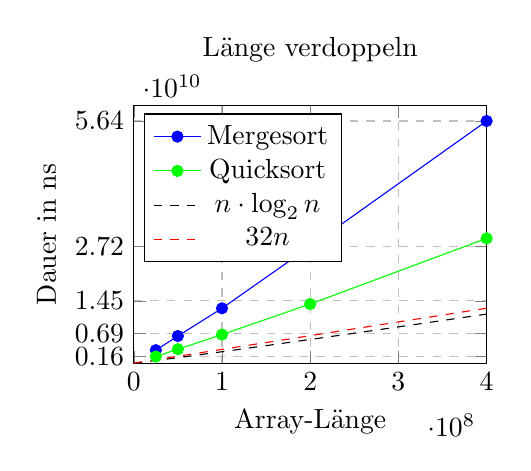
\begin{tikzpicture}
        \begin{axis}[
                title style={yshift=1.5ex},
                width=0.5\textwidth,
                height=0.4\textwidth,
                xlabel={Array-Länge},
                ylabel={Dauer in ns},
                title={Länge verdoppeln},
                xmin=0, xmax=4 * 10^8,
                ymin=0, ymax=6*10^10,
                grid=both,
                grid style=dashed,
                legend pos=north west,
                ytick={1609541400,6854920900,14495472700,27203738300,56441153000},
                % xtick={2^21,2^23,2^24,2^25},
                % xticklabels={$2^{21}$, $2^{23}$, $2^{24}$, $2^{25}$},
                % scaled x ticks=false,
                % scaled y ticks=false,
            ]
            \MergesortMaxArrayVerdoppelnMesswerte
            \QuicksortMaxArrayVerdoppelnMesswerte
            % n*log2(n)
            \addplot[black, dashed,domain=1:4e8, samples=100] {x*log2(x)};
            \addlegendentry{$n \cdot \log_2 n$}
            % n
            \addplot[red, dashed,domain=1:4e8, samples=100] {32*x};
            \addlegendentry{$32n$}
            % % log2(n)
            % \addplot[green, domain=1e7:4e8, samples=100] {log2(x)};
            % \addlegendentry{$\log_2 n$}
        \end{axis}
    \end{tikzpicture}%
}

\newcommand{\GrundlegendeLaufzeitenAbhaengigVonDerArraygroesseDiagrammB}{%
    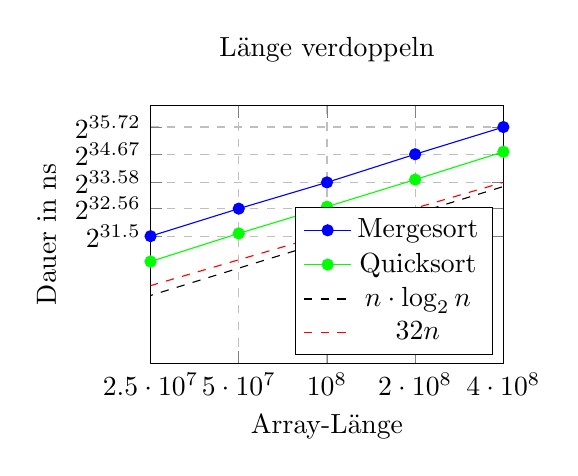
\begin{tikzpicture}
        \begin{axis}[
                title style={yshift=1.5ex},
                width=0.5\textwidth,
                height=0.4\textwidth,
                xlabel={Array-Länge},
                ylabel={Dauer in ns},
                title={Länge verdoppeln},
                xmin=2.5*10^7, xmax=4*10^8,
                ymin=10^8, ymax=1*10^11,
                grid=both,
                grid style=dashed,
                legend pos=south east,
                xmode=log,
                log basis x=10,
                xtick=data,
                xticklabels={$2.5\cdot10^7$, $5\cdot10^7$, $10^8$, $2\cdot10^8$, $4\cdot10^8$},
                ymode=log,
                log basis y=2,
                ytick=data,
                % xtick={2^21,2^23,2^24,2^25},
                % xticklabels={$2^{21}$, $2^{23}$, $2^{24}$, $2^{25}$},
                % scaled x ticks=false,
                % scaled y ticks=false,
            ]
            \MergesortMaxArrayVerdoppelnMesswerte
            \QuicksortMaxArrayVerdoppelnMesswerte
            % n*log2(n)
            \addplot[black, dashed,domain=1e7:4e8, samples=100] {x*log2(x)};
            \addlegendentry{$n \cdot \log_2 n$}
            % n
            \addplot[red, dashed,domain=1:4e8, samples=100] {32*x};
            \addlegendentry{$32n$}
            % % 64*x - 1000000000
            % \addplot[gray, dashed,domain=2*10^7:4e8, samples=100] {64*x - 10^9};
            % \addlegendentry{$64 \cdot n - 10^9$}
        \end{axis}
    \end{tikzpicture}%
}

\newcommand{\GrundlegendeLaufzeitenAbhaengigVonDerArraygroesseDiagrammC}{%
    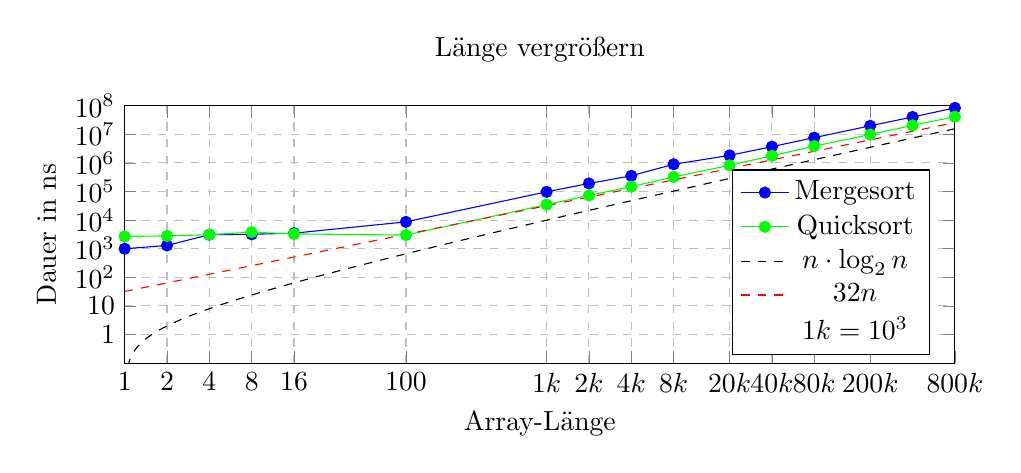
\begin{tikzpicture}
        \begin{axis}[
                title style={yshift=1.5ex},
                width=1\textwidth,
                height=0.4\textwidth,
                xlabel={Array-Länge},
                ylabel={Dauer in ns},
                title={Länge vergrößern},
                xmin=1, xmax=800000,
                ymin=0.1, ymax=1*10^8,
                grid=both,
                grid style=dashed,
                legend pos=south east,
                xmode=log,
                log basis x=10,
                %xtick=data,
                xtick={1,2,4,8,16,100,1000,2000,4000,8000,20000,40000,80000,200000,800000},
                xticklabels={
                        $1$,$2$,$4$,$8$,$16$,
                        $100$,$1k$,
                        $2k$,$4k$,$8k$,
                        $20k$,$40k$,$80k$,
                        $200k$,$800k$
                    },
                ymode=log,
                log basis y=10,
                ytick={1,10,10^2,10^3,10^4,10^5,10^6,10^7,10^8},
                yticklabels={$1$,$10$,$10^{2}$,$10^{3}$,$10^{4}$,$10^{5}$,$10^{6}$,$10^{7}$,$10^{8}$},
                % scaled x ticks=false,
                % scaled y ticks=false,
            ]
            \MergesortArrayVerdoppeln
            \QuicksortArrayVerdoppeln
            % n*log2(n)
            \addplot[black, dashed,domain=1:800000, samples=1000] {x*log2(x)};
            \addlegendentry{$n \cdot \log_2 n$}
            % n
            \addplot[red, dashed,domain=1:800000, samples=100] {32*x};
            \addlegendentry{$32n$}
            \addlegendimage{empty legend}
            \addlegendentry{$1k = 10^3$}
        \end{axis}
    \end{tikzpicture}%
}

\newcommand{\EinflussDesListentypsDiagrammA}{%
    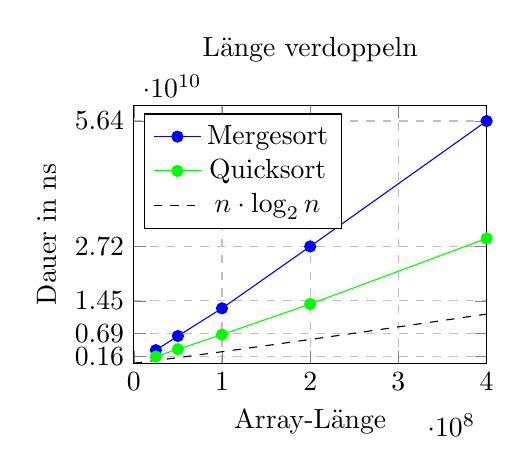
\begin{tikzpicture}
        \begin{axis}[
                title style={yshift=1.5ex},
                width=0.5\textwidth,
                height=0.4\textwidth,
                xlabel={Array-Länge},
                ylabel={Dauer in ns},
                title={Länge verdoppeln},
                xmin=0, xmax=4 * 10^8,
                ymin=0, ymax=6*10^10,
                grid=both,
                grid style=dashed,
                legend pos=north west,
                ytick={1609541400,6854920900,14495472700,27203738300,56441153000},
                % xtick={2^21,2^23,2^24,2^25},
                % xticklabels={$2^{21}$, $2^{23}$, $2^{24}$, $2^{25}$},
                % scaled x ticks=false,
                % scaled y ticks=false,
            ]
            \MergesortMaxArrayVerdoppelnMesswerte
            \QuicksortMaxArrayVerdoppelnMesswerte
            % n*log2(n)
            \addplot[black, dashed,domain=1:4e8, samples=100] {x*log2(x)};
            \addlegendentry{$n \cdot \log_2 n$}
        \end{axis}
    \end{tikzpicture}%
}

\newcommand{\EinflussDesListentypsDiagrammB}{%
    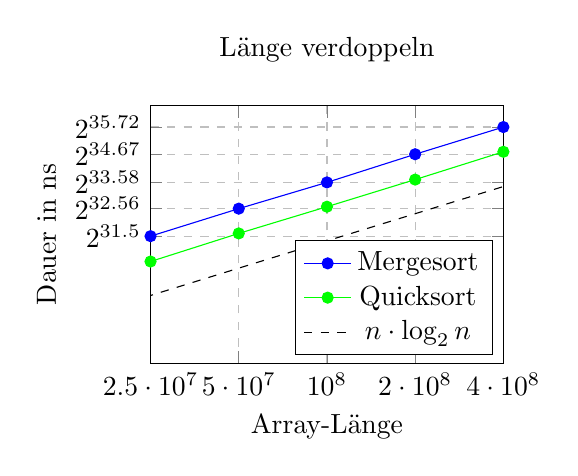
\begin{tikzpicture}
        \begin{axis}[
                title style={yshift=1.5ex},
                width=0.5\textwidth,
                height=0.4\textwidth,
                xlabel={Array-Länge},
                ylabel={Dauer in ns},
                title={Länge verdoppeln},
                xmin=2.5*10^7, xmax=4*10^8,
                ymin=10^8, ymax=1*10^11,
                grid=both,
                grid style=dashed,
                legend pos=south east,
                xmode=log,
                log basis x=10,
                xtick=data,
                xticklabels={$2.5\cdot10^7$, $5\cdot10^7$, $10^8$, $2\cdot10^8$, $4\cdot10^8$},
                ymode=log,
                log basis y=2,
                ytick=data,
                % xtick={2^21,2^23,2^24,2^25},
                % xticklabels={$2^{21}$, $2^{23}$, $2^{24}$, $2^{25}$},
                % scaled x ticks=false,
                % scaled y ticks=false,
            ]
            \MergesortMaxArrayVerdoppelnMesswerte
            \QuicksortMaxArrayVerdoppelnMesswerte
            % n*log2(n)
            \addplot[black, dashed,domain=1e7:4e8, samples=100] {x*log2(x)};
            \addlegendentry{$n \cdot \log_2 n$}
        \end{axis}
    \end{tikzpicture}%
}